% Provenance (never printed): cycle 3 / 6e "La planete Terre" (structure of
% the globe: crust, mantle, core); see sources/book1/PROVENANCE.md. Book 1,
% grade 6, chapter 4.
% Vocabulary guard: "magma" not before g7.2 ("molten rock"); P and S waves,
% Moho, core--mantle boundary and lithosphere belong to Book 2 (g11): the
% waves are told in prose, never defined; "seismometer" is defined in g7.3.
\chapter{地球内部}\label{ch:g6:inside-the-earth}

在俄罗斯遥远的西北部，靠近挪威边境，废弃建筑之间的地面上焊着一个金属盖。盖子下面，
有一个仅约 23~厘米宽的孔，笔直向下延伸超过 12~千米：
这是人类有史以来挖掘的最深孔洞。钻探它用了约 20~年。
钻探人员原本希望继续向下，但井底\omterm{def:g3:stones-pebbles-sand:rock}{岩石}的温度约为
180~摄氏度，几乎是预期的两倍：高温使钻头和钻管弯曲，
工程于 1992 年停止。然而地心
比这口井的井底深 \textbf{500 倍}以上。
我们如何得知地下深处有什么？
% ledger: sciam:kola-depth, sciam:kola-180C, earth:Rmean

\begin{omfigure}
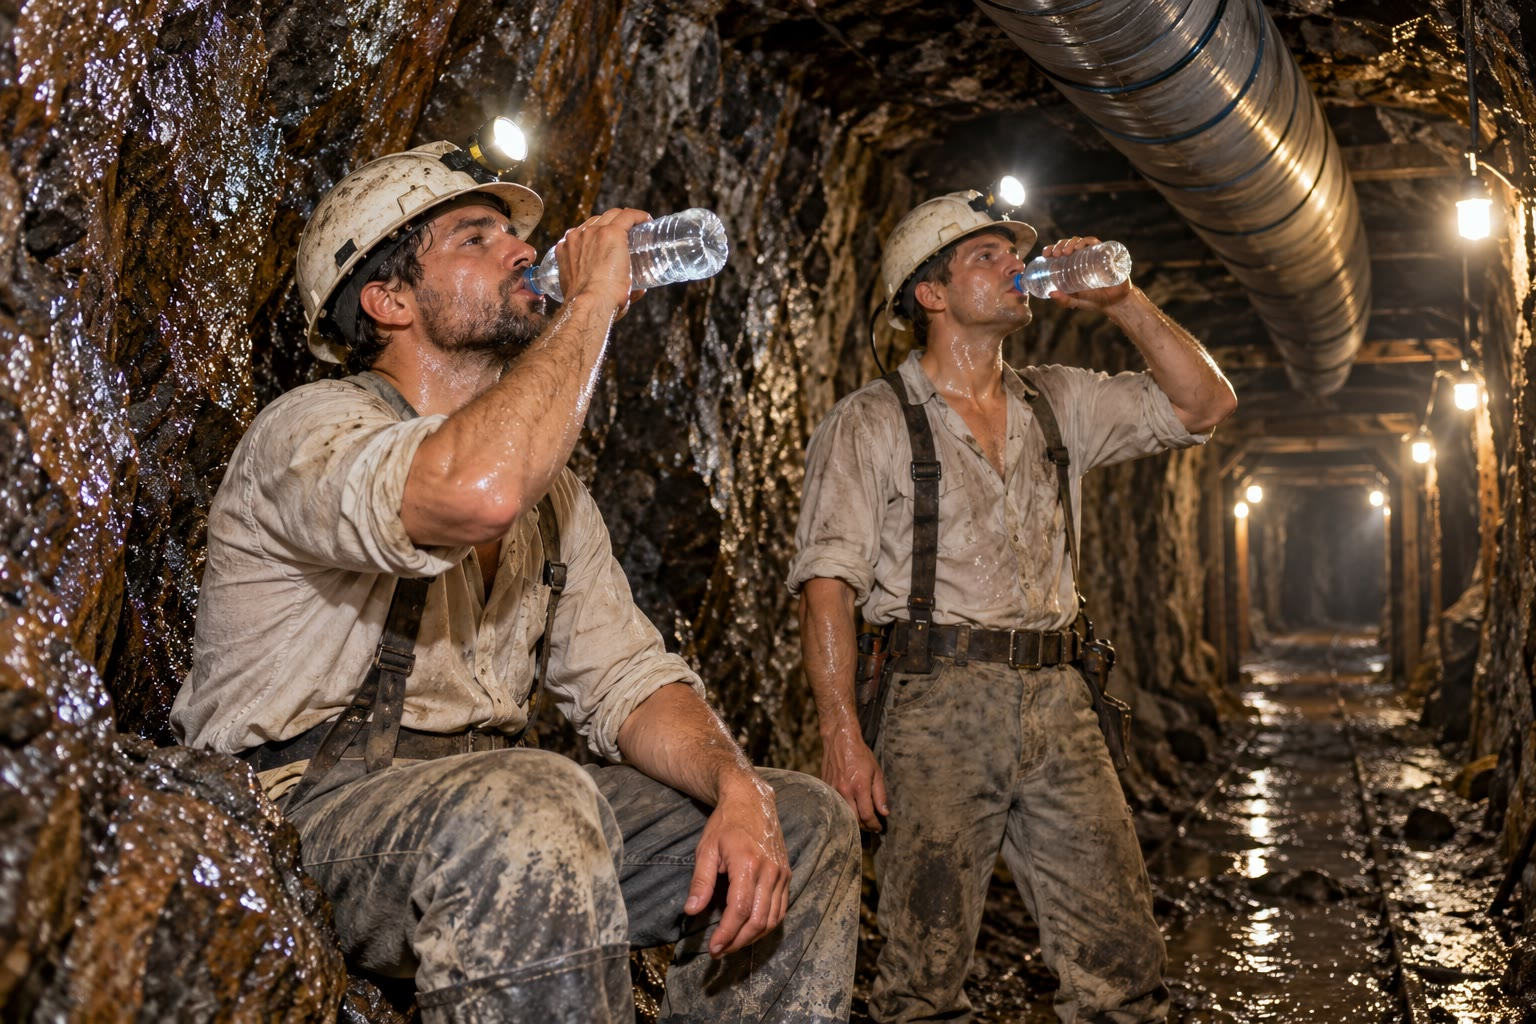
\includegraphics[width=0.62\linewidth]{images/book1/ai/g6-deep-mine.jpg}

{\small 矿工在地下数千米深处的炎热巷道中喝水。
（AI 插图。）}
\end{omfigure}

\begin{recall}
地球是一颗\omterm{def:g6:earth-a-planet:planet-types}{岩质行星}，是直径约 12\,742~千米的球体：其半径
即从表面到地心的距离，约为 6371~千米
（见\cref{ch:g6:earth-a-planet}）。地球的\omterm{def:g3:stones-pebbles-sand:rock}{岩石}分为三类：\omterm{def:g6:rocks-and-minerals:rock-families}{火成岩}、
\omterm{def:g6:rocks-and-minerals:rock-families}{沉积岩}和\omterm{def:g6:rocks-and-minerals:rock-families}{变质岩}（见\cref{ch:g6:rocks-and-minerals}）。在
\omterm{def:g4:volcanoes-earthquakes-first-look:volcano}{火山}处，熔融\omterm{def:g3:stones-pebbles-sand:rock}{岩石}从下方上升并喷出，形成\omterm{def:g4:volcanoes-earthquakes-first-look:eruption}{熔岩}；在
\omterm{def:g4:volcanoes-earthquakes-first-look:earthquake}{地震}中，地面发生震动（见\cref{ch:g4:volcanoes-earthquakes-first-look}）。
\end{recall}
% ledger: earth:Rmean

\section{人类挖得有多深？}

人类很早就向地下挖掘，以获取水、石料
和金属。挖得最深的有两类孔洞。

\textbf{矿井。}世界上最深的矿井是南非
约翰内斯堡附近的一座金矿，巷道向下延伸到地表以下超过 4~千米
处。那里的岩壁温度达到约 60~摄氏度：
矿井的降温方法是向下泵送数千吨与水混合的冰，
并用巨型风扇将空气吹过巷道。
% ledger: gwr:deepest-mine

\textbf{钻孔。}钻孔是由机器从地表钻入的一个狭窄孔洞，
没有人会下去。最深的钻孔是开篇故事中的
那口，为科学研究而钻于俄罗斯西北部的科拉半岛：
12\,262~米，即约 12.3~千米。
% ledger: sciam:kola-depth

这些深度看起来非常大。与地球的尺寸相比，它们
其实微不足道。下图把它们画在同一条带上，与最高
峰珠穆朗玛峰（8849~米）并列。
% ledger: tht:everest

\begin{omfigure}
\begin{tikzpicture}[yscale=0.27, xscale=1]
  % sea-level ground and the sky
  \fill[blue!6] (-0.2,0) rectangle (8.6,9.6);
  \fill[brown!35] (-0.2,0) rectangle (8.6,-13.4);
  \draw[thick, brown!60!black] (-0.2,0) -- (8.6,0);
  % depth axis
  \draw[->] (0,-13.4) -- (0,9.9) node[above, font=\scriptsize] {km};
  \foreach \y in {-12,-8,-4,0,4,8} \draw (-0.08,\y) -- (0.08,\y) node[left=2pt, font=\scriptsize] {\y};
  % Everest
  \fill[gray!55] (1.0,0) -- (2.2,8.849) -- (3.4,0) -- cycle;
  \draw[dashed, gray] (0,8.849) -- (2.2,8.849);
  \node[font=\scriptsize, right] at (2.35,8.6) {珠穆朗玛峰，高 8.8~km};
  % deepest mine
  \draw[line width=2.2pt, black!70] (4.4,0) -- (4.4,-4);
  \draw[dashed, gray] (0,-4) -- (4.4,-4);
  \node[font=\scriptsize, right, align=left] at (4.5,-3.6) {最深矿井，\\ 超过 4~km};
  % Kola borehole
  \draw[line width=0.7pt, red!75!black] (6.8,0) -- (6.8,-12.262);
  \draw[dashed, gray] (0,-12.262) -- (6.8,-12.262);
  \node[font=\scriptsize, left, align=right, red!60!black] at (6.7,-10.6) {最深钻孔，\\ 12.3~km};
  % break and the centre
  \draw[white, line width=3pt] (-0.3,-13.15) -- (8.7,-12.75);
  \draw (-0.3,-13.35) -- (8.7,-12.95);
  \draw (-0.3,-12.95) -- (8.7,-12.55);
  \node[font=\footnotesize, align=center] at (4.2,-16.2) {\ldots\ 地心位于地下 6371~km 处：\\
     在此比例下，它应位于本线以下约 17~米处。};
\end{tikzpicture}

{\small 高度与深度按同一比例绘制（1~厘米代表 3.7~千米），
从\omterm{def:g4:world-physical-map:altitude}{海平面}算起。带状图中的断口遮住了几乎全部通往
地心的路程。}
% ledger: tht:everest, gwr:deepest-mine, sciam:kola-depth, earth:Rmean
\end{omfigure}

\begin{method}[比较深度与地球半径]\label{met:g6:inside-the-earth:percent}
\begin{enumerate}
  \item 将深度和半径换算为同一单位（千米）。
  \item 用深度除以半径，再乘以 100：这样得到
        深度占通往地心全程的百分比。
  \item 要说明地心比该深度深多少倍，用半径除以
        该深度。
\end{enumerate}
\end{method}

\begin{example}[最深的钻孔]\label{ex:g6:inside-the-earth:kola}
钻孔深 12.3~千米，地球半径为 6371~千米。
$12.3 \div 6371 \approx 0.0019$，$0.0019 \times 100 = 0.19$：
钻孔大约走完了通往地心路程的 \textbf{0.2~\%}。反过来算，
$6371 \div 12.3 \approx 518$：地心比
钻孔底部深 500~倍以上。

对最深的矿井，深约 4~千米：$4 \div 6371 \approx 0.0006$，即
0.06~\%：比钻孔浅得多，约为钻孔的三分之一。
% ledger: sciam:kola-depth, earth:Rmean, gwr:deepest-mine
\end{example}

因此，没有人见过、触摸过或取样过地球的深部。
我们对它的认识主要来自其他线索，尤其是
\omterm{def:g4:volcanoes-earthquakes-first-look:earthquake}{地震}波（见第~\ref{sec:g6:inside-the-earth:waves}~节）。

\section{地壳、地幔和地核}

地球是分层的，有点像煮熟的鸡蛋：外面是一层薄而脆的
壳，中间是厚厚的“蛋白”，中心是“蛋黄”。
% ledger: usgs:layers-egg

\begin{omfigure}
\begin{tikzpicture}
  % a boiled egg cut in half
  \begin{scope}
    \fill[white] (0,0) ellipse (1.25 and 1.6);
    \draw[brown!50!black, line width=1.6pt] (0,0) ellipse (1.25 and 1.6);
    \fill[yellow!70!orange] (0,-0.15) circle (0.72);
    \node[font=\scriptsize, anchor=west] (s) at (1.8,1.3) {蛋壳};
    \draw[gray] (s.west) -- (1.0,0.98);
    \node[font=\scriptsize, anchor=west] (w) at (1.8,0.4) {蛋白};
    \draw[gray] (w.west) -- (0.95,0.4);
    \node[font=\scriptsize, anchor=west] (y) at (1.8,-0.5) {蛋黄};
    \draw[gray] (y.west) -- (0.5,-0.4);
    \node[font=\small] at (0,-2.0) {煮熟的鸡蛋};
  \end{scope}
  \draw[->, thick, gray] (3.0,0) -- (4.2,0);
  % the Earth, not to scale
  \begin{scope}[xshift=6.2cm]
    \fill[orange!45!red!45] (0,0) circle (1.55);
    \fill[orange!75!yellow] (0,0) circle (0.95);
    \fill[yellow!55] (0,0) circle (0.42);
    \draw[brown!50!black, line width=1.6pt] (0,0) circle (1.55);
    \node[font=\scriptsize, anchor=west] (c) at (1.95,1.3) {地壳};
    \draw[gray] (c.west) -- (1.12,1.07);
    \node[font=\scriptsize, anchor=west] (m) at (1.95,0.55) {地幔};
    \draw[gray] (m.west) -- (1.2,0.5);
    \node[font=\scriptsize, anchor=west] (o) at (1.95,-0.2) {外核};
    \draw[gray] (o.west) -- (0.7,-0.2);
    \node[font=\scriptsize, anchor=west] (i) at (1.95,-0.9) {内核};
    \draw[gray] (i.west) -- (0.15,-0.25);
    \node[font=\small] at (0,-2.0) {地球（未按比例绘制）};
  \end{scope}
\end{tikzpicture}

{\small 地球与煮熟的鸡蛋的比较。与蛋黄不同，\omterm{def:g6:inside-the-earth:layers}{地核}分为
两部分。本图中\omterm{def:g6:inside-the-earth:layers}{地壳}画得比实际厚得多，
按比例绘制的图见下文。}
% ledger: usgs:layers-egg
\end{omfigure}

\begin{definition}[地球的分层]\label{def:g6:inside-the-earth:layers}
地球由三个主要圈层组成，从表面到中心依次为：
\begin{itemize}
  \item \emph{地壳}\index{地壳}，是最外层的薄层固体\omterm{def:g3:stones-pebbles-sand:rock}{岩石}，
        厚度为几千米至几十千米；
  \item \emph{地幔}\index{地幔}，是厚厚的一层炽热、致密的
        固态\omterm{def:g3:stones-pebbles-sand:rock}{岩石}，深度约延伸至 2900~千米；
  \item \emph{地核}\index{地核}，由金属构成，主要是铁，并含有一些
        镍，从约 2900~千米深处直到地心。地核分为两部分：
        \emph{外核}\index{外核}为液态，
        \emph{内核}\index{内核}为位于中心的固体球体，
        半径约 1220~千米。
\end{itemize}
% ledger: usgs:layers-egg, usgs:crust-thickness, data:prem, earth:Rmean
\end{definition}

下图按\emph{比例}绘制各圈层，各分界面
由\omterm{def:g4:volcanoes-earthquakes-first-look:earthquake}{地震}波测定。

\begin{omfigure}
\pgfplotstableread{figdata/out/grade-6-earth_layers-disc.dat}\disctab
\pgfplotstablegetelem{0}{r_cm}\of\disctab \let\rE\pgfplotsretval
\pgfplotstablegetelem{1}{r_cm}\of\disctab \let\rOC\pgfplotsretval
\pgfplotstablegetelem{2}{r_cm}\of\disctab \let\rIC\pgfplotsretval
\begin{minipage}[c]{0.43\linewidth}\centering
\begin{tikzpicture}
  \fill[orange!45!red!45] (0,0) circle (\rE cm);
  \fill[orange!75!yellow] (0,0) circle (\rOC cm);
  \fill[yellow!55] (0,0) circle (\rIC cm);
  \draw[brown!50!black, line width=0.45pt] (0,0) circle (\rE cm);
  
  \draw[gray, thin] (-0.25,\rE) rectangle (0.25,\rE-0.12);
  
  \node[font=\scriptsize, align=center, inner sep=0pt] at (0,0) {内 \\ 核};
  \node[font=\scriptsize, align=center] at (0,1.03) {外 \\ 核};
  \node[font=\scriptsize] at (0,2.12) {地幔};
  \draw[<-, font=\scriptsize] (1.98,1.98) -- (2.3,2.75) node[above, align=center] {地壳 \\ （薄如发丝）};
\end{tikzpicture}
\end{minipage}\hfill
\begin{minipage}[c]{0.55\linewidth}\centering
\begin{tikzpicture}[yscale=0.034, xscale=0.55]
  % the top 100 km enlarged: ocean on the left, continent and a range on the right
  \fill[orange!45!red!45] (0,0) rectangle (12,-100);
  \fill[blue!25] (0,0) rectangle (4,-4);
  \fill[brown!45] (0,-4) rectangle (4,-9);                 % oceanic crust 5 km
  \fill[brown!60] (4,0) -- (4,-9) -- (5,-30) -- (8,-30) -- (9,-100) -- (11,-100) -- (11.4,-30) -- (12,-30) -- (12,0) -- cycle;
  \fill[brown!60] (8.6,0) -- (10,5) -- (11.4,0) -- cycle;   % the range (not to scale above ground)
  \draw[red!75!black, line width=0.8pt] (6.2,0) -- (6.2,-12.262);
  \draw[thin] (0,0) rectangle (12,-100);
  \foreach \y in {0,-20,-40,-60,-80,-100} \draw (0,\y) -- (-0.2,\y) node[left, font=\scriptsize] {\pgfmathparse{-\y}\pgfmathprintnumber{\pgfmathresult}};
  \node[font=\scriptsize, rotate=90] at (-2.0,-50) {深度（km）};
  \node[font=\scriptsize, align=center] at (2,-44) {大洋 \\ 地壳，\\ 5~km};
  \draw[->, thin] (2,-29) -- (2,-8);
  \node[font=\scriptsize, align=center] at (6.6,-21) {大陆 \\ 地壳，30~km};
  \node[font=\scriptsize, align=center] at (10.0,-50) {山脉 \\ 之根，\\ 深达 \\ 100~km};
  \node[font=\scriptsize, align=center, red!60!black] at (7.4,-6.5) {钻孔};
  \node[font=\scriptsize] at (4.5,-75) {地幔};
  \node[font=\scriptsize, blue!60!black] at (2,2.5) {海洋};
\end{tikzpicture}
\end{minipage}

\smallskip
{\small 左图：按比例绘制的剖开地球示意图；顶部的小灰框
标出右图所放大的部分。右图：顶部 100~千米，放大约
60~倍：\omterm{def:g2:water-on-earth:ocean}{海洋}之下\omterm{def:g6:inside-the-earth:layers}{地壳}较薄，\omterm{def:g3:continents-and-oceans:continent}{大陆}之下\omterm{def:g6:inside-the-earth:layers}{地壳}较厚，
高大\omterm{def:g4:world-physical-map:range}{山脉}之下\omterm{def:g6:inside-the-earth:layers}{地壳}最厚；纪录钻孔以红色标示。}
% ledger: data:prem, earth:Rmean, usgs:crust-thickness, sciam:kola-depth (figdata/grade-6/earth_layers.py)
\end{omfigure}

\begin{center}\small
\begin{tabular}{|l|c|c|c|l|}
\hline
\textbf{层} & \textbf{起始深度（千米）} & \textbf{终止深度（千米）} & \textbf{厚度（千米）} & \textbf{物质组成} \\
\hline
\omterm{def:g6:inside-the-earth:layers}{地壳} & 0 & 5 至 100 & 5 至 100 & 固体\omterm{def:g3:stones-pebbles-sand:rock}{岩石} \\
\omterm{def:g6:inside-the-earth:layers}{地幔} & \omterm{def:g6:inside-the-earth:layers}{地壳}底部 & 2891 & 约 2860 & 固体\omterm{def:g3:stones-pebbles-sand:rock}{岩石}，温度很高 \\
\omterm{def:g6:inside-the-earth:layers}{外核} & 2891 & 5150 & 约 2260 & 液体金属 \\
\omterm{def:g6:inside-the-earth:layers}{内核} & 5150 & 6371（地心） & 约 1220 & 固体金属 \\
\hline
\end{tabular}
\end{center}
% ledger: data:prem, usgs:crust-thickness, usgs:layers-egg, earth:Rmean (figdata/grade-6/earth_layers.py, main table)

\textbf{\omterm{def:g6:inside-the-earth:layers}{地壳}}是我们唯一能够站立其上、向下挖掘的一层。与其他各层相比，它非常薄：
\omterm{def:g2:water-on-earth:ocean}{海洋}之下，它只有约 5~千米厚；
\omterm{def:g3:continents-and-oceans:continent}{大陆}之下平均约 30~千米；高大\omterm{def:g4:world-physical-map:range}{山脉}之下，
如阿尔卑斯山，其底部可深达 100~千米，形似
牙根。即便是纪录钻孔，深 12.3~千米，也未达到平均\omterm{def:g3:continents-and-oceans:continent}{大陆}\omterm{def:g6:inside-the-earth:layers}{地壳}厚度的一半。按比例绘制的图中，\omterm{def:g6:inside-the-earth:layers}{地壳}
比圆盘周围的线还细。
% ledger: usgs:crust-thickness, sciam:kola-depth

\textbf{\omterm{def:g6:inside-the-earth:layers}{地幔}}是最厚的一层：它从\omterm{def:g6:inside-the-earth:layers}{地壳}底部
向下延伸至 2891~千米深处，约占通往地心路程的 45~\%。其\omterm{def:g3:stones-pebbles-sand:rock}{岩石}
为固体，但温度很高，密度比\omterm{def:g6:inside-the-earth:layers}{地壳}\omterm{def:g3:stones-pebbles-sand:rock}{岩石}更大。在数百万年间，
\omterm{def:g6:inside-the-earth:layers}{地幔}中部分炽热\omterm{def:g3:stones-pebbles-sand:rock}{岩石}能够极其缓慢地蠕动，
如同很稠的糊状物。
% ledger: data:prem, usgs:layers-egg, usgs:lithosphere-80km

\textbf{\omterm{def:g6:inside-the-earth:layers}{地核}}从 2891~千米深处开始，一直延伸到地心。它
不是\omterm{def:g3:stones-pebbles-sand:rock}{岩石}，而是金属：一种铁与镍的合金，密度几乎
是\omterm{def:g6:inside-the-earth:layers}{地幔}的两倍。其外层是\emph{液体}：一片由熔融金属组成的
\omterm{def:g2:water-on-earth:ocean}{海洋}，深逾 2000~千米。其内层从 5150~千米深处直至地心，
是一个\emph{固体}金属球，半径约 1220~千米，直径约为月球的 70~\%。地球自转时，\omterm{def:g6:inside-the-earth:layers}{外核}中的液体金属
流动，这一运动产生了地球磁场，
正是让指南针指针转动的那个磁场。
% ledger: data:prem, usgs:layers-egg, earth:Rmean, planet:Moon.diameter

越深，密度越大。水的密度为 1~克每立方
厘米：\omterm{def:g6:inside-the-earth:layers}{地壳}\omterm{def:g3:stones-pebbles-sand:rock}{岩石}的密度是水的 2.6 至 2.9 倍，
\omterm{def:g6:inside-the-earth:layers}{地幔}底部\omterm{def:g3:stones-pebbles-sand:rock}{岩石}的密度超过水的 5~倍，地心金属的密度约为水的
13~倍（见下图）。最重的物质位于中心，最轻的位于顶部：地球按密度分层排列，从轻的\omterm{def:g6:inside-the-earth:layers}{地壳}到重的金属\omterm{def:g6:inside-the-earth:layers}{地核}。
% ledger: data:prem


\begin{omfigure}
\begin{tikzpicture}
  \begin{axis}[omrecord, width=0.86\linewidth, height=5.4cm,
      xmin=0, xmax=6371, ymin=0, ymax=14,
      xlabel={地表以下深度（千米）},
      ylabel={密度（克每 cm$^3$）},
      xtick={0,1000,2000,3000,4000,5000,6000},
      scaled x ticks=false, x tick label style={/pgf/number format/1000 sep={}},
      clip=false]
    \fill[orange!45!red!20] (axis cs:24.4,0) rectangle (axis cs:2891,14);
    \fill[orange!75!yellow!35] (axis cs:2891,0) rectangle (axis cs:5149.5,14);
    \fill[yellow!30] (axis cs:5149.5,0) rectangle (axis cs:6371,14);
    \addplot[very thick, black] table[x=depth_km, y=rho] {figdata/out/grade-6-earth_layers-profile.dat};
    \node[font=\scriptsize] at (axis cs:1450,12.5) {地幔};
    \node[font=\scriptsize] at (axis cs:4020,4.5) {外核};
    \node[font=\scriptsize] at (axis cs:5760,4.5) {内核};
    \node[font=\scriptsize, align=left, anchor=west] at (axis cs:80,1.4) {地壳：2.6 至 2.9};
  \end{axis}
\end{tikzpicture}

{\small 地球各深度处的密度，由根据\omterm{def:g4:volcanoes-earthquakes-first-look:earthquake}{地震}测量建立的参考模型给出。
密度由约 5.6 跃升至约
9.9~克每 cm$^3$，此处即\omterm{def:g6:inside-the-earth:layers}{地幔}\omterm{def:g3:stones-pebbles-sand:rock}{岩石}让位于
\omterm{def:g6:inside-the-earth:layers}{地核}金属的界面。}
% ledger: data:prem (figdata/grade-6/earth_layers.py, part profile)
\end{omfigure}

\begin{inthelab}[玻璃杯中的分层（课堂上，与教师一起）]
教师依次、缓慢地向一只高玻璃杯中倒入：
蜂蜜、滴入一滴墨水的水和食用油。
无论按怎样的顺序倒入，过一会儿，蜂蜜沉在
底部，水在中间，油在最上层：每种液体都
位于较轻者之下、较重者之上。摇动后，玻璃杯变得浑浊；
静置后，它又会自行分层。地球以同样的方式分层：密度最大的物质，即\omterm{def:g6:inside-the-earth:layers}{地核}的金属，位于中心，最轻的\omterm{def:g3:stones-pebbles-sand:rock}{岩石}位于最上层。
\end{inthelab}


\begin{remark}[地壳到底有多薄？]\label{rem:g6:inside-the-earth:thin-crust}
若用直径 30~厘米的教学\omterm{def:g3:continents-and-oceans:globe}{地球仪}来表示，\omterm{def:g3:continents-and-oceans:continent}{大陆}\omterm{def:g6:inside-the-earth:layers}{地壳}（30~千米）
约厚 0.7~毫米，\omterm{def:g2:water-on-earth:ocean}{海洋}\omterm{def:g6:inside-the-earth:layers}{地壳}（5~千米）约相当于
一张纸的厚度。\omterm{def:g6:inside-the-earth:layers}{地壳}厚度不到地球半径的百分之一的一半：
$30 \div 6371 \approx 0.0047$，也就是 0.47~\%。
% ledger: usgs:crust-thickness, earth:Rmean
\end{remark}

\section{地震波如何揭示其余部分}\label{sec:g6:inside-the-earth:waves}

既然没有人挖到比 12~千米更深的地方，我们如何画出\omterm{def:g6:inside-the-earth:layers}{地核}？答案
来自\omterm{def:g4:volcanoes-earthquakes-first-look:earthquake}{地震}。\omterm{def:g4:volcanoes-earthquakes-first-look:earthquake}{地震}使地面震动时，波从震源
向各个方向传出，并\emph{穿过}整个地球传播，就像
敲门声穿过墙壁那样。世界各地的许多仪器记录每种波的到达时刻（你将在
\cref{ch:g7:earthquakes}中见到它们）。
% ledger: data:prem

波在不同的物质中传播速度并不相同。当波
到达两层之间的分界面时，其速度会突然改变：有些波
被反射回来，另一些则在穿过时发生弯折，有点像光进入
水中。通过在全球各地台站测量许多次\omterm{def:g4:volcanoes-earthquakes-first-look:earthquake}{地震}中波的到达时间，科学家已经找到了这些分界面的位置，
以及各层是固体还是液体。\omterm{def:g4:volcanoes-earthquakes-first-look:earthquake}{地震}学家把两种主要的波称为
\emph{P 波}（较快的一种，使\omterm{def:g3:stones-pebbles-sand:rock}{岩石}前后推拉）和
\emph{S 波}（较慢的一种，使\omterm{def:g3:stones-pebbles-sand:rock}{岩石}左右晃动）；
后续分册将对它们作深入研究。S 波有一个显著的特性：它
不能穿过液体传播。

\begin{omfigure}
\begin{tikzpicture}
  \begin{axis}[omrecord, width=0.86\linewidth, height=5.4cm,
      xmin=0, xmax=6371, ymin=0, ymax=14.5,
      xlabel={地表以下深度（km）},
      ylabel={传播速度（千米每秒）},
      xtick={0,1000,2000,3000,4000,5000,6000},
      scaled x ticks=false, x tick label style={/pgf/number format/1000 sep={}},
      clip=false]
    \fill[orange!45!red!20] (axis cs:24.4,0) rectangle (axis cs:2891,14.5);
    \fill[orange!75!yellow!35] (axis cs:2891,0) rectangle (axis cs:5149.5,14.5);
    \fill[yellow!30] (axis cs:5149.5,0) rectangle (axis cs:6371,14.5);
    \addplot[very thick, blue!70!black] table[x=depth_km, y=vp] {figdata/out/grade-6-earth_layers-profile.dat};
    \addplot[very thick, red!75!black] table[x=depth_km, y=vs] {figdata/out/grade-6-earth_layers-profile.dat};
    \node[font=\scriptsize, blue!70!black, anchor=south] at (axis cs:1300,12.9) {P 波（较快）};
    \node[font=\scriptsize, red!75!black, anchor=north] at (axis cs:1500,6.1) {S 波（较慢）};
    \node[font=\scriptsize, red!75!black, align=center, fill=white, fill opacity=0.8, text opacity=1] at (axis cs:4020,1.9) {S 波：0\\（液体）};
    \node[font=\scriptsize] at (axis cs:4020,13.6) {外核};
    \node[font=\scriptsize] at (axis cs:5760,13.6) {内核};
    \node[font=\scriptsize] at (axis cs:1450,1.5) {地幔};
  \end{axis}
\end{tikzpicture}

{\small 两类\omterm{def:g4:volcanoes-earthquakes-first-look:earthquake}{地震}波在各深度处的速度，
取自同一参考模型。在\omterm{def:g6:inside-the-earth:layers}{外核}中 S 波消失：其速度
为零，因为\omterm{def:g6:inside-the-earth:layers}{外核}是液体。}
% ledger: data:prem (figdata/grade-6/earth_layers.py, part profile)
\end{omfigure}

从左往右读图：在\omterm{def:g6:inside-the-earth:layers}{地幔}中，两类波
的速度都随深度增加而越来越快。在 2891~km 处，S 波消失，
P 波速度突然减小：这是液态\omterm{def:g6:inside-the-earth:layers}{外核}的顶部。在
5150~km 处，P 波速度再次增大，S 波重新出现：这是
固态\omterm{def:g6:inside-the-earth:layers}{内核}。
% ledger: data:prem

\begin{history}[英格·莱曼与内核]
\begin{minipage}[c]{0.72\linewidth}
20 世纪 30 年代初，\omterm{def:g4:volcanoes-earthquakes-first-look:earthquake}{地震}学家认为地球只有两层：包着液态\omterm{def:g6:inside-the-earth:layers}{地核}的固态\omterm{def:g6:inside-the-earth:layers}{地幔}。丹麦\omterm{def:g4:volcanoes-earthquakes-first-look:earthquake}{地震}学家英格·莱曼研究了
1929 年袭击新西兰的一次强震的波，这些波被远方的台站记录下来。有些波
到达的地方，若\omterm{def:g6:inside-the-earth:layers}{地核}完全是液态的，这些波本不该到达。
1936 年她发表的一篇文章，题目简单地叫作“P\,$'$''”，
她提出一个解释：液态\omterm{def:g6:inside-the-earth:layers}{地核}内部还有一个较小的
\emph{固态\omterm{def:g6:inside-the-earth:layers}{内核}}，它把这些波送回。她谦逊地写道，
数据“相当不足”，难以断定，但这种解释“似乎可能”，
并请其他研究者加以检验。他们照做了，如今固态\omterm{def:g6:inside-the-earth:layers}{内核}已成为
每一个地球参考模型的一部分，本章图中所用的参考模型即是其中之一。
% ledger: nbi:lehmann-1936
\end{minipage}\hfill
\begin{minipage}[c]{0.24\linewidth}\centering
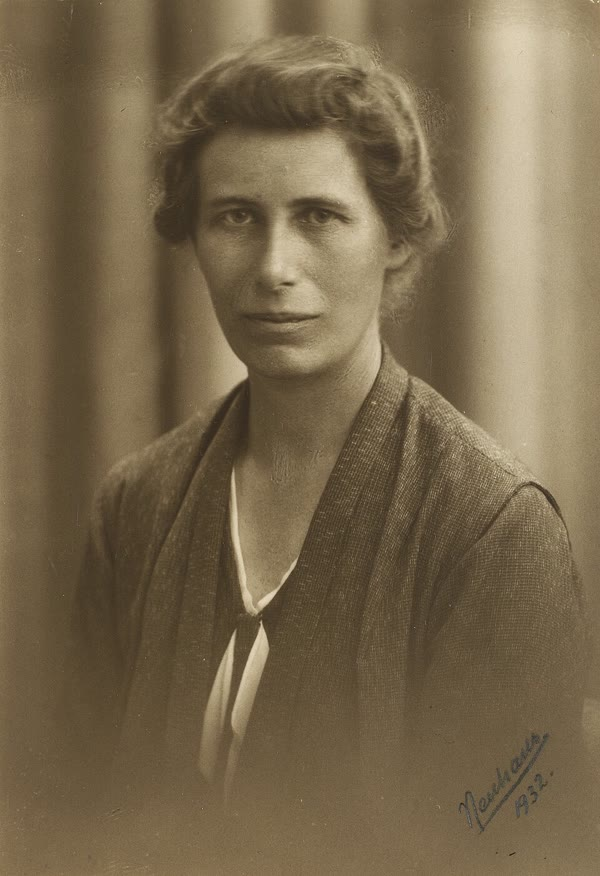
\includegraphics[width=\linewidth]{images/book1/g6-inge-lehmann.jpg}\\[2pt]
{\footnotesize 英格·莱曼，1932 年。（照片：Even Neuhaus，公有领域，
经由维基共享资源。）}
% ledger: commons:inge-lehmann
\end{minipage}
\end{history}

\section{越深越热}

每一座深矿井和每一个深钻孔都显示同一规律：越往深处，
\omterm{def:g3:stones-pebbles-sand:rock}{岩石}越热。在最深的矿井中，井壁\omterm{def:g3:stones-pebbles-sand:rock}{岩石}温度可达
约 60~摄氏度，深度超过 4~km；在创纪录的深钻孔底部，
即 12.3~km 深处，\omterm{def:g3:stones-pebbles-sand:rock}{岩石}温度约为 180~摄氏度。
% ledger: gwr:deepest-mine, sciam:kola-180C

近地表处，温度以相当稳定的速率上升。在
美国，科学家收集了 284 个钻孔的测量数据，
其中大部分深于 600~m。平均而言，
\textbf{每深入 1 千米，温度升高 29~摄氏度}：东部约为每千米 25~摄氏度，
西部则为 34。但速率因地而异，差别很大：在这些钻孔中，
速率在每千米 6~摄氏度至
69~摄氏度之间变化。
% ledger: usgs:gradient-29

\begin{omfigure}
\begin{tikzpicture}
  \begin{axis}[omrecord, omdepth, width=0.78\linewidth, height=5.6cm,
      xmin=0, xmax=160, ymin=0, ymax=2,
      xlabel={岩石温度（$^\circ$C）},
      ylabel={深度（km）},
      ytick={0,0.5,1,1.5,2},
      yticklabel style={/pgf/number format/fixed},
      legend pos=north east, legend cell align=left,
            legend style={font=\scriptsize},
      clip=false]
    \addplot[forget plot, name path=lo, thin, gray] table[x=t_low, y=depth_km] {figdata/out/grade-6-earth_layers-geotherm.dat};
    \addplot[forget plot, name path=hi, thin, gray] table[x=t_high, y=depth_km] {figdata/out/grade-6-earth_layers-geotherm.dat};
    \addplot[forget plot, gray!20] fill between[of=lo and hi];
    \addplot[forget plot, thick, blue!70!black] table[x=t_east, y=depth_km] {figdata/out/grade-6-earth_layers-geotherm.dat};
    \addplot[forget plot, very thick, black] table[x=t_mean, y=depth_km] {figdata/out/grade-6-earth_layers-geotherm.dat};
    \addplot[forget plot, thick, red!75!black] table[x=t_west, y=depth_km] {figdata/out/grade-6-earth_layers-geotherm.dat};
    \addlegendimage{area legend, fill=gray!20, draw=gray}
    \addlegendentry{每千米 6 至 69 $^\circ$C：全部钻孔}
    \addlegendimage{thick, blue!70!black}\addlegendentry{每千米 25 $^\circ$C：东部}
    \addlegendimage{very thick, black}\addlegendentry{每千米 29 $^\circ$C：平均}
    \addlegendimage{thick, red!75!black}\addlegendentry{每千米 34 $^\circ$C：西部}
  \end{axis}
\end{tikzpicture}

{\small 温度随深度（向下）的变化。地面起始温度为
15~$^\circ$C，分别按平均速率（29，黑色）、东部和西部平均值（25 和 34）
以及全部实测范围（6 至 69，灰色带）绘制。
实测数据可达约 2~km。}
% ledger: usgs:gradient-29, planet:Earth.Tmean (figdata/grade-6/earth_layers.py, part geotherm)
\end{omfigure}

\begin{method}[某深度处的温度]\label{met:g6:inside-the-earth:temperature}
\begin{enumerate}
  \item 测量近地表地面的温度。
  \item 将深度（以千米计）乘以速率（以摄氏度每千米计），
        所得即为温度升高的量。
  \item 将两者相加。仅在速率已被测量过的范围内使用此方法，
        即仅限几千米的范围。
\end{enumerate}
\end{method}

\begin{example}[深两千米处]\label{ex:g6:inside-the-earth:two-km}
地面温度为 15~$^\circ$C，温度每千米升高 29~度。
在 2~千米深处：温度升高 $2 \times 29 = 58$ 度，因此 $15 + 58 = 73~^\circ$C：
比最热的洗澡水还热，已经热得无法触碰。
% ledger: usgs:gradient-29, planet:Earth.Tmean
\end{example}

能否将同样的速率一直用到地心？不能。若按每千米 29~度计算，
地心温度约为 185\,000~度，这是不可能的，原因是
在最初几千米测得的速率并不适用于深处，那里的温度必须升高得慢得多。科学家另用一种方法估计\omterm{def:g6:inside-the-earth:layers}{地核}温度：
在实验室中，他们把微小的铁颗粒夹在两颗金刚石之间，
施加相当于空气压强数百万倍的压力，
再用激光加热，直至熔化。由此发现，
在固态\omterm{def:g6:inside-the-earth:layers}{内核}的边缘，温度约为
\textbf{6000~摄氏度}，然而\omterm{def:g6:inside-the-earth:layers}{内核}中的铁仍保持固态，因为那里的压强
相当于空气压强的 330 万倍，使其无法熔化。
% ledger: esrf:core-6000C, usgs:gradient-29

\begin{remark}[热而仍为固态]\label{rem:g6:inside-the-earth:pressure}
物质受到的挤压越大，熔化所需的温度就越高。
\omterm{def:g6:inside-the-earth:layers}{地幔}温度很高，却仍是固态；\omterm{def:g6:inside-the-earth:layers}{外核}是液态；\omterm{def:g6:inside-the-earth:layers}{内核}
温度更高，却又变为固态，因为它受到的挤压最大。
物质是否熔化，取决于温度\emph{和}压强。
% ledger: esrf:core-6000C, data:prem
\end{remark}

\section{练习}

\begin{exercise}[$\star$]\label{exo:g6:inside-the-earth:1}
依次写出地球的四个圈层，从地表到
地心。哪一层是液态？哪些层由金属构成？
\end{exercise}

\begin{exercise}[$\star$]\label{exo:g6:inside-the-earth:2}
判断下列说法是否正确，并改正错误的说法。
(a) \omterm{def:g2:water-on-earth:ocean}{海洋}下的\omterm{def:g6:inside-the-earth:layers}{地壳}比\omterm{def:g3:continents-and-oceans:continent}{大陆}下的\omterm{def:g6:inside-the-earth:layers}{地壳}更厚。
(b) \omterm{def:g6:inside-the-earth:layers}{地核}由\omterm{def:g3:stones-pebbles-sand:rock}{岩石}构成。
(c) \omterm{def:g6:inside-the-earth:layers}{内核}是固态的。
(d) 人类钻探过的最深钻孔深约 12~千米。
\end{exercise}

\begin{exercise}[$\star$]\label{exo:g6:inside-the-earth:3}
根据圈层表，(a) \omterm{def:g6:inside-the-earth:layers}{地核}从多深处开始？
(b) \omterm{def:g6:inside-the-earth:layers}{内核}从多深处开始？(c) \omterm{def:g6:inside-the-earth:layers}{外核}的
厚度是多少？
\end{exercise}

\begin{exercise}[$\star$]\label{exo:g6:inside-the-earth:4}
人们常把地球比作一个煮熟的鸡蛋。请抄写并补全：“
蛋壳像\ldots，蛋白像\ldots{}，蛋黄则像
\ldots{}。但与蛋黄不同，\ldots{}分为两部分：液态的
\ldots{}和固态的\ldots{}。”
\end{exercise}

\begin{exercise}[$\star\star$]\label{exo:g6:inside-the-earth:5}
珠穆朗玛峰高 8.849~千米，地球半径为 6371~千米。以
半径的百分比表示，珠穆朗玛峰高多少？结果保留两位小数。
从远处看，地球表面是否十分崎岖？
\end{exercise}

\begin{exercise}[$\star\star$]\label{exo:g6:inside-the-earth:6}
\omterm{def:g3:continents-and-oceans:continent}{大陆}\omterm{def:g6:inside-the-earth:layers}{地壳}平均厚 30~千米，大洋\omterm{def:g6:inside-the-earth:layers}{地壳}平均厚
5~千米。(a) \omterm{def:g3:continents-and-oceans:continent}{大陆}\omterm{def:g6:inside-the-earth:layers}{地壳}的厚度是大洋\omterm{def:g6:inside-the-earth:layers}{地壳}的多少倍？(b) 在高大的
\omterm{def:g4:world-physical-map:range}{山脉}之下，\omterm{def:g6:inside-the-earth:layers}{地壳}厚度可达 100~千米。
这一厚度是大洋\omterm{def:g6:inside-the-earth:layers}{地壳}的多少倍？
\end{exercise}

\begin{exercise}[$\star\star$]\label{exo:g6:inside-the-earth:7}
某地区地面温度为 12~$^\circ$C，温度每千米升高
25~度。求下列深度的温度：(a) 1~千米处，(b) 在
1.5~千米处，(c) 2~千米处的温度各为多少？
\end{exercise}

\begin{exercise}[$\star\star$]\label{exo:g6:inside-the-earth:8}
在某钻孔中，近地表\omterm{def:g3:stones-pebbles-sand:rock}{岩石}为 14~$^\circ$C，在
2~千米深处为 74~$^\circ$C。温度每千米
升高多少度？这一速率是否介于本章测量的东部与西部
平均值之间？
\end{exercise}

\begin{exercise}[$\star\star$]\label{exo:g6:inside-the-earth:9}
利用波速图。(a) 紧靠\omterm{def:g6:inside-the-earth:layers}{地核}上方的 P 波
（约 2890~千米深处）以及紧靠\omterm{def:g6:inside-the-earth:layers}{地核}顶部之下的速度分别是多少？
(b) S 波速度为零的深度范围在哪里？(c) 这说明该层
具有什么性质？
\end{exercise}

\begin{exercise}[$\star\star$]\label{exo:g6:inside-the-earth:10}
创纪录的钻孔深 12.3~千米。(a) 它穿过的深度占平均\omterm{def:g3:continents-and-oceans:continent}{大陆}\omterm{def:g6:inside-the-earth:layers}{地壳}
（30~千米）厚度的百分之几？(b) 它是否到达了\omterm{def:g6:inside-the-earth:layers}{地幔}？
\end{exercise}

\begin{exercise}[$\star\star\star$]\label{exo:g6:inside-the-earth:11}
利奥说：“在近地表处，温度每千米升高 29~度，
所以在深 6371~千米的地心处，温度必定为
$15 + 29 \times 6371$ 度。”(a) 计算利奥给出的数值。(b) 将其与
实验室中测得的\omterm{def:g6:inside-the-earth:layers}{内核}边缘温度相比较。(c) 利奥的推理
错在哪里？
\end{exercise}

\begin{exercise}[$\star\star\star$]\label{exo:g6:inside-the-earth:12}
整个地球的平均密度约为 5.5~克每立方
厘米（见\cref{ch:g6:earth-a-planet}），但\omterm{def:g6:inside-the-earth:layers}{地壳}\omterm{def:g3:stones-pebbles-sand:rock}{岩石}的密度
只有 2.6 到 2.9。(a) 这说明深处的物质
具有什么特点？(b) 利用密度图，哪些圈层中的密度处处高于 5.5？(c) 为什么重金属位于
地心而不在地表，为什么是合理的？
\end{exercise}

\section{问题：按比例的地心之旅}

\begin{problem}[{周末问题——按比例的直径 2~米地球模型：各圈层、
最深的钻孔与炽热的内部，按比例绘制}]
\label{pb:g6:inside-the-earth:1}
% ledger: earth:Rmean, data:prem, usgs:crust-thickness, sciam:kola-depth, tht:everest, usgs:gradient-29, gwr:deepest-mine, esrf:core-6000C
为学校开放日，一个班级要制作一个剖开一半的地球模型，
模型尽可能大：\omterm{def:g3:continents-and-oceans:equator}{半球}的平面是一个直径 2~米的圆盘，
上面画出各圈层。一切都必须按比例。已知：地球半径
6371~千米；\omterm{def:g6:inside-the-earth:layers}{外核}顶面深 2891~千米；\omterm{def:g6:inside-the-earth:layers}{内核}顶面深
5150~千米；\omterm{def:g3:continents-and-oceans:continent}{大陆}\omterm{def:g6:inside-the-earth:layers}{地壳}厚 30~千米；大洋\omterm{def:g6:inside-the-earth:layers}{地壳}厚 5~千米；珠穆朗玛峰高 8.849~千米；
创纪录的钻孔深 12.3~千米。

\medskip
\noindent\textbf{第一部分——模型。}
\begin{enumerate}
  \item 真实地球的直径是多少千米？
        写出模型的直径（以毫米为单位）。
  \item 模型上 1~毫米代表真实地球多少千米？
        （用真实直径除以模型直径。）
  \item 在模型上，珠穆朗玛峰高多少毫米？
        保留一位小数。
  \item 在模型上，创纪录的钻孔有多深？
        将它与模型表面到中心的距离作比较。
\end{enumerate}

\medskip
\noindent\textbf{第二部分——各圈层。}
\begin{enumerate}[resume]
  \item 学生应在模型表面以下多深处涂出\omterm{def:g6:inside-the-earth:layers}{外核}顶面？
        精确到最接近的毫米。
  \item 对\omterm{def:g6:inside-the-earth:layers}{内核}顶面，问题相同。
        模型上\omterm{def:g6:inside-the-earth:layers}{内核}的半径是多少？
  \item 沿模型的一条半径，哪一圈层占据的空间最大：
        \omterm{def:g6:inside-the-earth:layers}{地幔}、\omterm{def:g6:inside-the-earth:layers}{外核}还是\omterm{def:g6:inside-the-earth:layers}{内核}？给出其在模型上的
        厚度。
  \item \omterm{def:g3:continents-and-oceans:continent}{大陆}\omterm{def:g6:inside-the-earth:layers}{地壳}应涂多厚？保留一位小数。
        用画笔涂这样的厚度容易吗？
\end{enumerate}

\medskip
\noindent\textbf{第三部分——炽热的内部。}
\begin{enumerate}[resume]
  \item 学生按地表温度为
        15~$^\circ$C、每千米升温 29~摄氏度计算，写出 2~千米深处的温度。他们应写什么？
        2~千米深处位于模型表面以下多远处？
  \item 最深的矿井深度超过 4~千米。
        在模型上，该矿井比创纪录的钻孔更深还是更浅？
        相差约多少毫米？
  \item 在\omterm{def:g6:inside-the-earth:layers}{内核}边缘附近，标签上写着“
        约 6000~$^\circ$C，固态”。一位参观者感到惊讶：
        为什么\omterm{def:g6:inside-the-earth:layers}{外核}是液态，而温度更高的\omterm{def:g6:inside-the-earth:layers}{内核}却是固态？
  \item 大洋\omterm{def:g6:inside-the-earth:layers}{地壳}是最薄的圈层。
        在模型上它应有多厚（单位为毫米）？保留两位小数，
        并将其与一张纸的厚度（约 0.1~毫米）作比较。
\end{enumerate}
\end{problem}
